\documentclass[11pt]{article}
\usepackage[utf8]{inputenc}
\usepackage[spanish]{babel}
\usepackage{amsmath}
\usepackage{amsfonts}
\usepackage{amssymb}
\usepackage{graphicx}
\usepackage{tikz}
\usepackage[all]{xy}

\title{Automatizando el juego del triqui\\ Reporte del primer problema del curso\\ ``IA: Representación y solución de problemas''}
\author{Edgar Andrade}
\date{\today}

\begin{document}

\maketitle

\section{Introducción}

\noindent La automatización de juegos cuya resolución requiere algún grado de inteligencia fue una tarea muy relevante durante las primeras etapas de la inteligencia articial. Los juegos constituyen un muy buen conejillo de indias, toda vez que definen un entorno completamente regimentado y relativamente sencillo, fácilmente susceptible a la formalización. El juego del triqui (o tres-en-línea) es un ejemplar muy favorable a este respecto, sobre todo para la representación formal, y más bien sencilla, de un \emph{task environment} (REFERENCIA RUSSELL \& NORVIG SEC???), así como para ilustrar la metodología de búsqueda de soluciones en un espacio de estados.

El juego del triqui involucra dos jugadores, quienes hacen sus jugadas por turnos en un tablero de $3\times 3$. El primer jugador arranca poniendo $X$ en alguna casilla, luego el segundo pone una $O$ en alguna de las casillas vacías, luego vuelve el turno para el jugador 1 y así en adelante. El juego termina cuando no hay más casillas vacías o cuando alguno de los dos jugadores logra poner tres de sus figuras en línea (ver Figura \ref{fig:triqui}).

\begin{figure}
\begin{center}
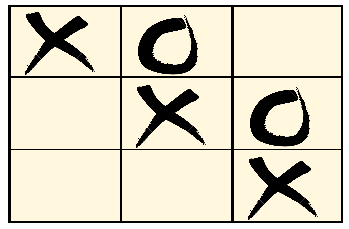
\includegraphics[scale=.2]{imagenes/triqui1}\hspace{.5cm}
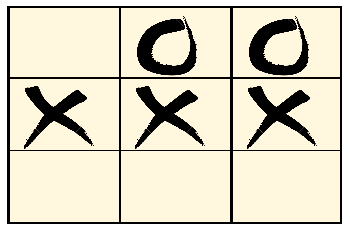
\includegraphics[scale=.2]{imagenes/triqui2}\hspace{.5cm}
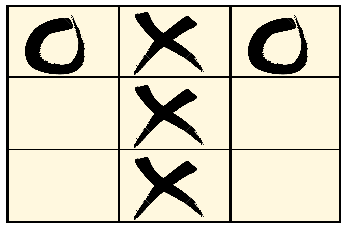
\includegraphics[scale=.2]{imagenes/triqui3}\hspace{.5cm}
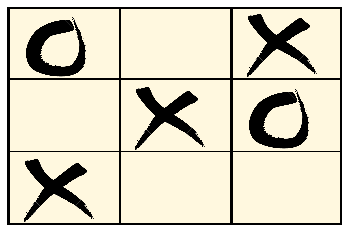
\includegraphics[scale=.2]{imagenes/triqui4}\hspace{.5cm}
\end{center}
\caption{Cuatro maneras de ganar el juego del triqui con las $X$. La victoria con las $O$ es similar.}\label{fig:triqui}
\end{figure}

Nuestro problema consiste en implementar un agente que sea competente para jugar al triqui. Este problema admite una solución completa, toda vez que el agente que implementamos nunca podrá ser derrotado. 

\section{Métodos}

\noindent La solución al problema requiere una definición formal previa a la implementación en python, que es la siguiente:

\begin{description}
\item[Estado inicial:] Situación del entorno desde el cual comienza el juego. En el caso del triqui, el estado inicial es el tablero vacío.
\item[Jugador($s$):] Define cuál jugador tiene el turno en el estado $s$, el cual puede ser $O$ o $X$.
\item[Posibles acciones($s$):] Descripción de las posibles acciones del $Jugador(s)$, dado un estado $s$. En este caso, poner o bien una $O$ o una $X$ en una casilla vacía.
\item[Función de transiciones($s$, $a$):] Descripción del entorno que resulta de la ejecución de la acción $a$ por el $Jugador(s)$ en el estado $s$. Junto con el estado inicial y las posibles acciones, la función de transiciones define el espacio de estados del juego.
\item[Prueba de objetivo($s$):] Permite determinar si el juego se termina cuando se obtiene el estado $s$.
\item[Función de utilidad($s$):] Definida sólo cuando el juego se termina en el estado s y especifica la recompensa de cada jugador en s. En el caso del triqui, asumiremos que el ganador obtiene 1, el perdedor 0 y, en caso de empate, ambos jugadores obtienen $\frac{1}{2}$.
\end{description}

Una vez implementado el problema así definido, se procedió a implementar la función \texttt{minmax-decision} (ver Figura \ref{fig:minmax}), la cual implementa el algoritmo minmax (REFERENCIA A R-Y-N, SEC???). Este algoritmo crea un árbol de estados, partiendo desde un estado dado $s$, atribuyéndole una utilidad a cada estado con base en los pagos generados por una condición final (ver función de utilidad arriba descrita). Los pagos para el jugador 1 con las $X$ son positivos, y los del jugador 2 con las $O$ son negativos, así que el primero buscará estados que maximicen la utilidad, mientras que el segundo buscará estados que la minimicen. Estas funciones definen el back-end de la aplicación.

\begin{figure}
\begin{center}
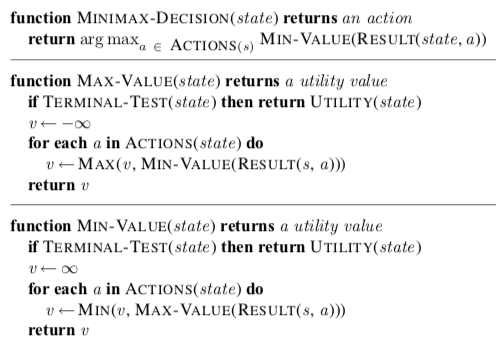
\includegraphics[scale=.5]{imagenes/busqueda-minmax}
\end{center}
\caption{Pseudo-código de las funciones que implementan la toma de decisiones del algoritmo minmax.}\label{fig:minmax}
\end{figure}

Como front-end, se impementó una página web usando la librería Dash de python, y fue desplegada en un servidor \textsc{ec2} en \textsc{aws}.

\section{Resultados}

\noindent\hspace{-1cm}\scalebox{0.9}{
\begin{tikzpicture}[level distance=2.5cm, level 1/.style={sibling distance=5cm}, level 2/.style={sibling distance=4cm}]
\node{\txt{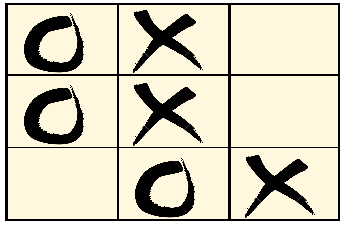
\includegraphics[scale=.2]{imagenes/tab122}\\ Valor minmax = 0\\ = max$\{-1, -1, 0\}$}}
    child { node [yshift=-1cm] {\txt{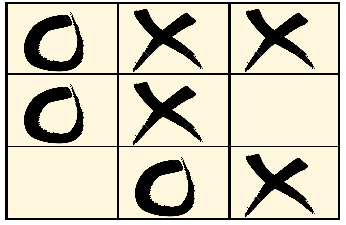
\includegraphics[scale=.2]{imagenes/tab1222}\\ Valor minmax = $-1$\\ = min$\{-1, 0, 0\}$}} 
			child { node [yshift=-1cm] {\txt{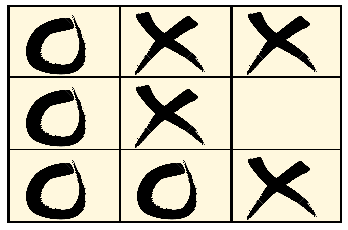
\includegraphics[scale=.2]{imagenes/tab12221}\\ Utilidad = $-1$}} }
		    	child { node {$\vdots$} }
    			child { node {$\vdots$} }
    		}
    	child { node {$\vdots$} }
    child { node [yshift=-1cm] {\txt{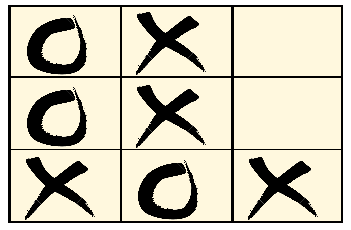
\includegraphics[scale=.2]{imagenes/tab1221}\\ Valor minmax = 0\\ = min$\{0, 1\}$}}
			child { node [yshift=-1cm] {\txt{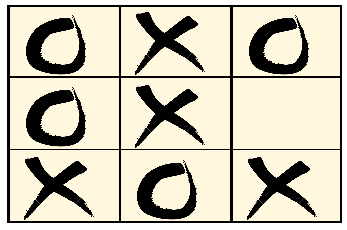
\includegraphics[scale=.2]{imagenes/tab12211}\\ Valor minmax = 0\\ = max$\{0\}$}} 
					child { node [yshift=-1cm] {\txt{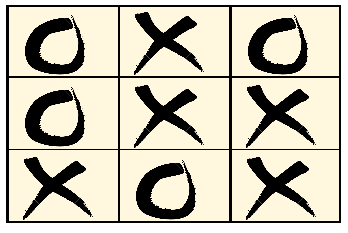
\includegraphics[scale=.2]{imagenes/tab122111}\\ Utilidad = 0}} }
				}
			child { node [yshift=-1cm] {\txt{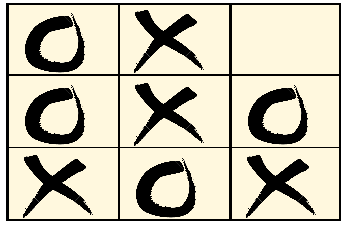
\includegraphics[scale=.2]{imagenes/tab12212}\\ Valor minmax = 1\\ = max$\{1\}$} } 
					child { node [yshift=-1cm] {\txt{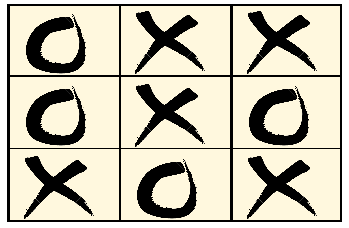
\includegraphics[scale=.2]{imagenes/tab122121}\\ Utilidad = 1}} }
				}
		}
	;
\end{tikzpicture}
} % end scalebox


POR QUÉ ESTE AGENTE NO PUEDE SER DERROTADO???

\section{Discusión}

\section{Conclusiones}

REFERENCIAS

\end{document}